\newpage
\section{Parallelisation}
\label{parallel}
\indent
\par 

\subsection{Sequential Profiling}
Prior to parallelisation every step of the linear algebra expression was profiled to identify potencial hotspots. Since the best parallel linear algebra version turned out to be the CSC version, special attention is added to it when compared to the CSR version. \par 
Table \ref{table:profile_seq} displays the profiler results for  the CSC version with the largest TPC-H dataset in test - 32GB, namely the percentage of overall time for each operation present in expression \ref{eq:tpch_1}.

\begin{table}[H]
\centering
\footnotesize
  \begin{tabular}{ | L{1cm} | L{1.25cm} |  L{1.2cm} |  L{1.3cm} |  L{1.6cm} | L{1cm} |  }
    \hline
    LA Version	&	Projection	&	Selection	&	Projection . Selection	&	(Projection .Selection). Quantity	&	Bang	\\ \hline
Seq. CSC	&	23.93\%	&	43.38\%	&	10.89\%	&	18.12\%	&	3.68\%	\\ \hline
  \end{tabular}
     \caption{Profiling results for the sequential CSC linear algebra version, for TPC-H 32GB dataset, for the evaluation platform.}
     \label{table:profile_seq}
\end{table}

As shown in table \ref{table:profile_seq}, the most time consuming operations are the selection and the projection (Khratri-Rao operation). Further efforts to reduce the selection overhead are discussed in subsection \ref{optimization_selection}. \par 

\subsection{Parallel Experimental Results and Analysis}

To parallelise both linear algebra versions, in a multicore system, we opted by OpenMP version 4.0.
Using the CSC format in the linear algebra version the algorithms offer good parallelisation opportunities, since each column has at most one element. 

To parallelise with the CSR format the algorithms are more challenging. \par 

Figure \ref{fig:time_la_vs_ra_parallel} presents the measured execution times for a wide range of datasets, and for both linear and relational algebra approaches. The presented values were selected through the K-Best technique, with K=3 from 50 samples. For the linear algebra approach we present the the best execution times for the best CSR and CSC formats, namely the CSC format version.\par

As shown, the parallel linear algebra approach is faster than the parallel relational algebra, although larger TPC-H datasets reduce the gain from the linear algebra approach. Further algorithm optimisation will be discussed in  subsection \ref{optimization_selection}.\par 

\begin{figure}[H]
\centering
\caption{TPC-H benchmark simplified query-1 time for solution analysis for different scale factors, between parallel linear and relational algebra approaches.}
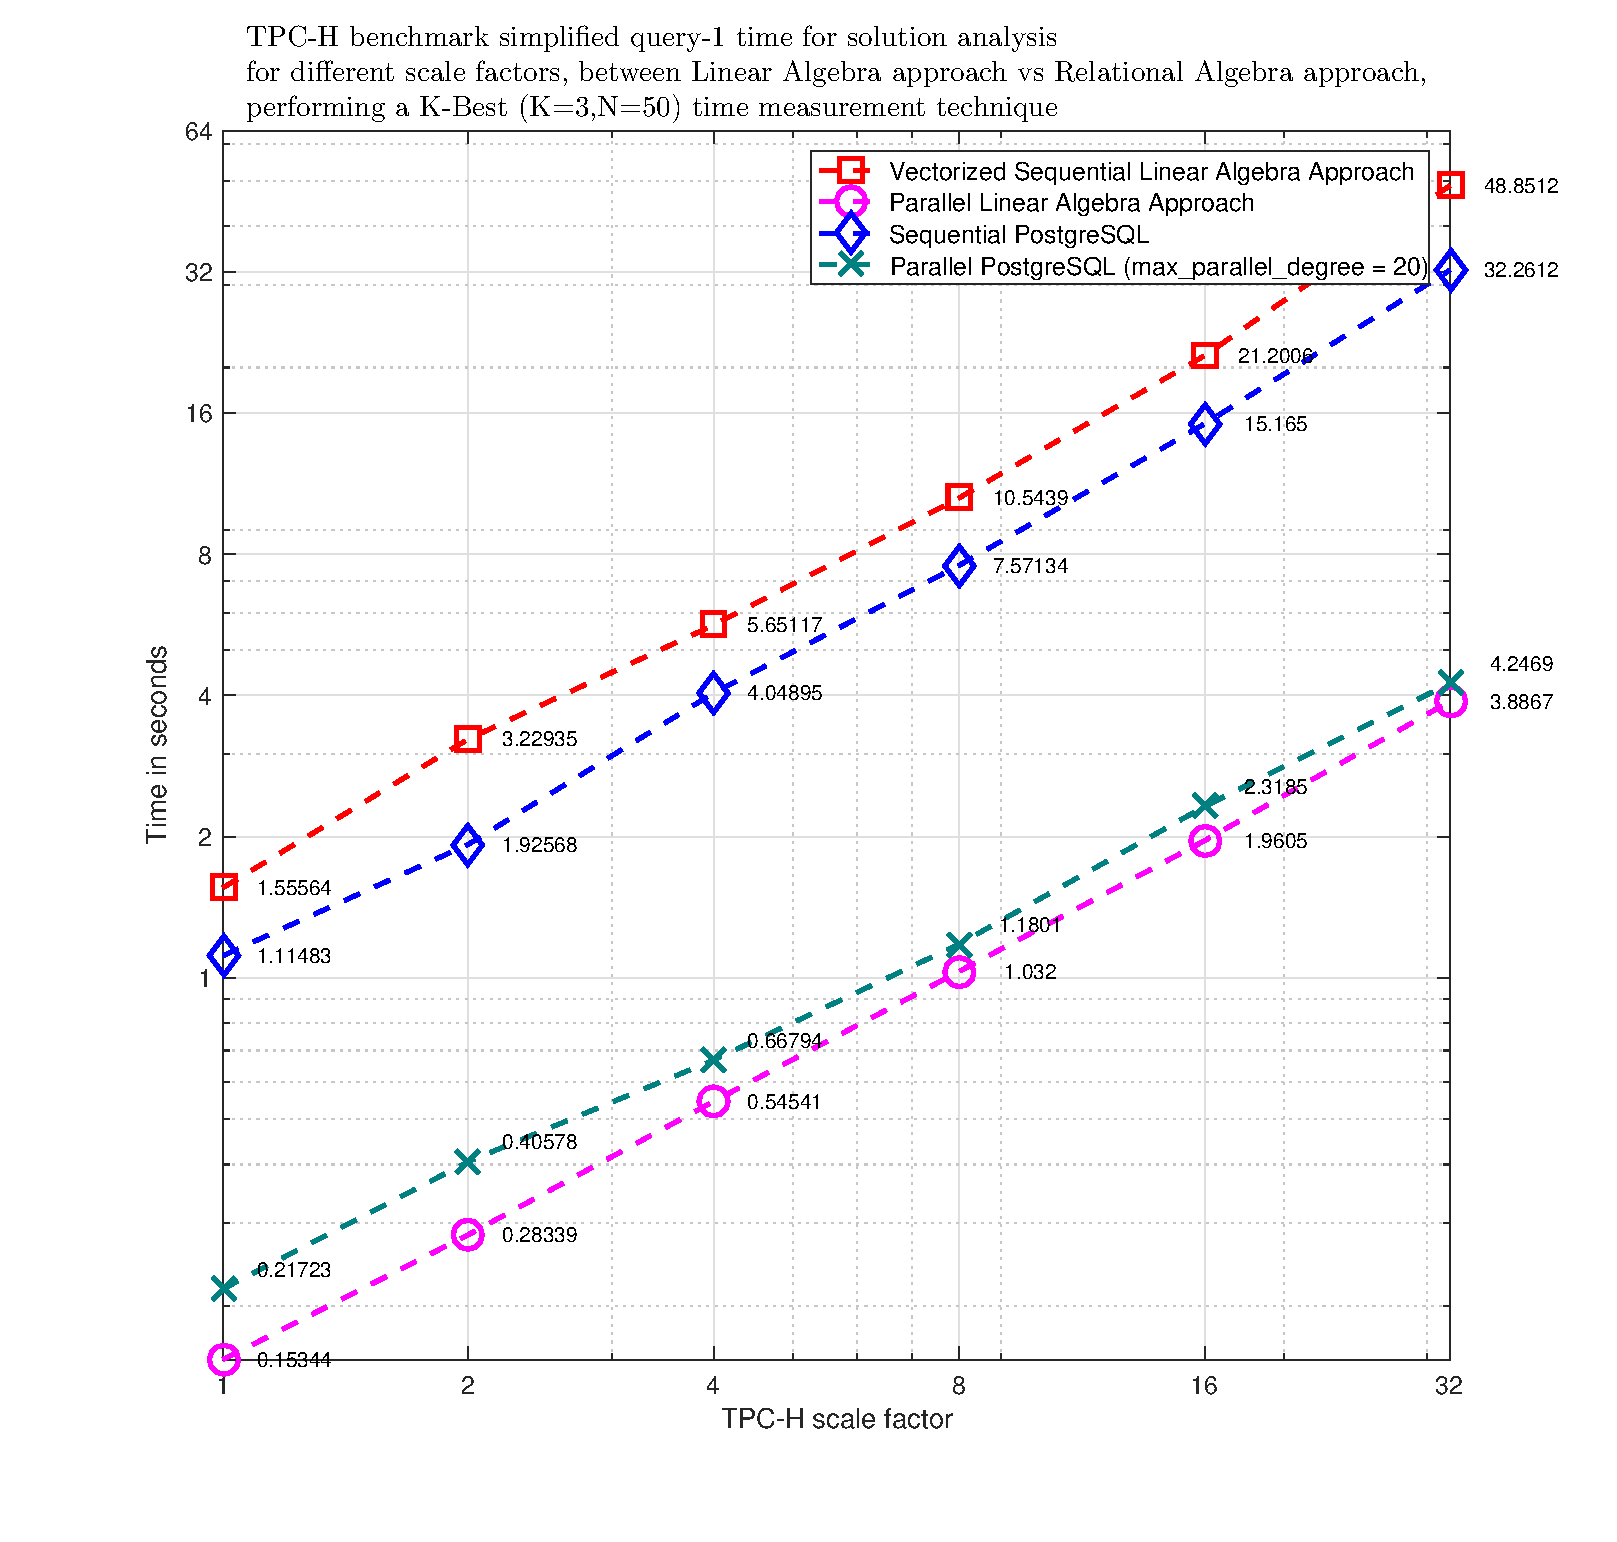
\includegraphics[width=1\columnwidth]{eps/TIME_LA_vs_RA_parallel.eps}
\label{fig:time_la_vs_ra_parallel}
\end{figure}

\subsection{Further Selection Algorithm Optimisation}
\label{optimization_selection}

Further profiling was made to better identify the potential bottlenecks. Table \ref{table:profile_par} compares both sequential and parallel linear algebra versions. The projection operation has decreased the percentage of overall time to complete the operation. However, the selection operation has increased its overall time percentage  to almost half the overall value. \par 


\begin{table}[H]
\centering
\footnotesize
  \begin{tabular}{ | L{1cm} | L{1.25cm} |  L{1.2cm} |  L{1.3cm} |  L{1.6cm} | L{1cm} |  }
    \hline
    LA Version	&	Projection	&	Selection	&	Projection . Selection	&	(Projection .Selection). Quantity	&	Bang	\\ \hline
Seq. CSC	&	23.93\%	&	43.38\%	&	10.89\%	&	18.12\%	&	3.68\%	\\ \hline
Par. CSC	&	13.62\%	&	46.83\%	&	11.49\%	&	16.74\%	&	3.51\%	\\ \hline

  \end{tabular}
     \caption{Profiling results for the parallel CSC linear algebra version, for TPC-H 32GB dataset, for the evaluation platform.}
     \label{table:profile_par}
\end{table}

After a careful examination of a portion the C source code for the CSC version selection, in listing \ref{selection_code_old}, further algorithm optimisations can be made. 

\newpage
\lstinputlisting[caption=Portion of the C source code for the CSC linear algebra version selection algorithm, label=selection_code_old]{src/selection_old.c} 

Taking as example the TPC-H 32GB dataset, and the shipdate matrix, with dimension $(\ m\ \times\ n\ ), namely $(\ 2,531\ $\times\ 192,000,551\ )$, to compute the selection result, in the worst case scenario, it is necessary to realize $(n * 2) = 384,001,102 $ string comparisons. However, by analysing table \ref{table:dataset_info}, from the 384,001,102 string comparisons only 2,531 distinct strings will be tested.\par 
 Listing \ref{selection_code_new} avoids repetitive string comparisons  by adding an additional auxiliar array (of size n), resulting in a worst case scenario of  $(m * 2) = 5,062 $ string comparisons and $n = 192,000,551 $ integer comparisons.\par
 This solution resolves two distinct problems:  the excessive overhead of accessing a large amount and repetitive string comparisons, and the improvement of this solution with bigger datasets. 
 The additional overhead of producing an auxiliar array gets diminished with the increase of the dataset  and consequently the required comparisons.  The larger the dataset, the better. 

\lstinputlisting[caption=Portion of the C source code for the CSC linear algebra version selection algorithm, label=selection_code_new]{src/selection_new.c} 

Table \ref{table:profile_par_new} compares three parallel linear algebra versions: the sequential, the parallel, and an optimised parallel version. The selection operation largely diminished its percentage overall time making it possible for the overall time to be averagely distributed among operations. \par 

\begin{table}[H]
\centering
\footnotesize
  \begin{tabular}{ | L{1cm} | L{1.25cm} |  L{1.2cm} |  L{1.3cm} |  L{1.6cm} | L{1cm} |  }
    \hline
    LA Version	&	Projection	&	Selection	&	Projection . Selection	&	(Projection .Selection). Quantity	&	Bang	\\ \hline
Seq. CSC	&	23.93\%	&	43.38\%	&	10.89\%	&	18.12\%	&	3.68\%	\\ \hline
Par. CSC	&	13.62\%	&	46.83\%	&	11.49\%	&	16.74\%	&	3.51\%	\\ \hline
Optimized Par. CSC	&	10.47\%	&	20.10\%	&	25.86\%	&	34.60\%	&	8.98\%	\\ \hline
  \end{tabular}
     \caption{Profiling results for the selection algorithm optimised parallel CSC linear algebra version, for TPC-H 32GB dataset, for the evaluation platform.}
     \label{table:profile_par_new}
\end{table}

\subsection{Final Parallel Experimental Results}

Figure \ref{fig:time_la_vs_ra_parallel_v2} presents the measured execution times for a wide range of datasets, and both linear and relational algebra approaches.   The presented values were selected through the K-Best technique, with K=3 from 50 samples. 
For the linear algebra approach we present the the best solution with the CSC format, in the optimised parallel version.\par
As shown, the parallel linear algebra solution in both versions is faster than the parallel relational algebra, and the speedup was stable for whole range of  TPC-H datasets.\par 
Figure \ref{fig:speedup_la_vs_ra_parallel} plots the obtained speedups between sequential LA and parallel LA versions, and between the parallel LA and RA versions.

\begin{figure}[H]
\centering
\caption{TPC-H benchmark simplified query-1 time for solution analysis for different scale factors, between parallel linear and relational algebra approaches, in which linear algebra approach states the selection algorithm optimisation.}
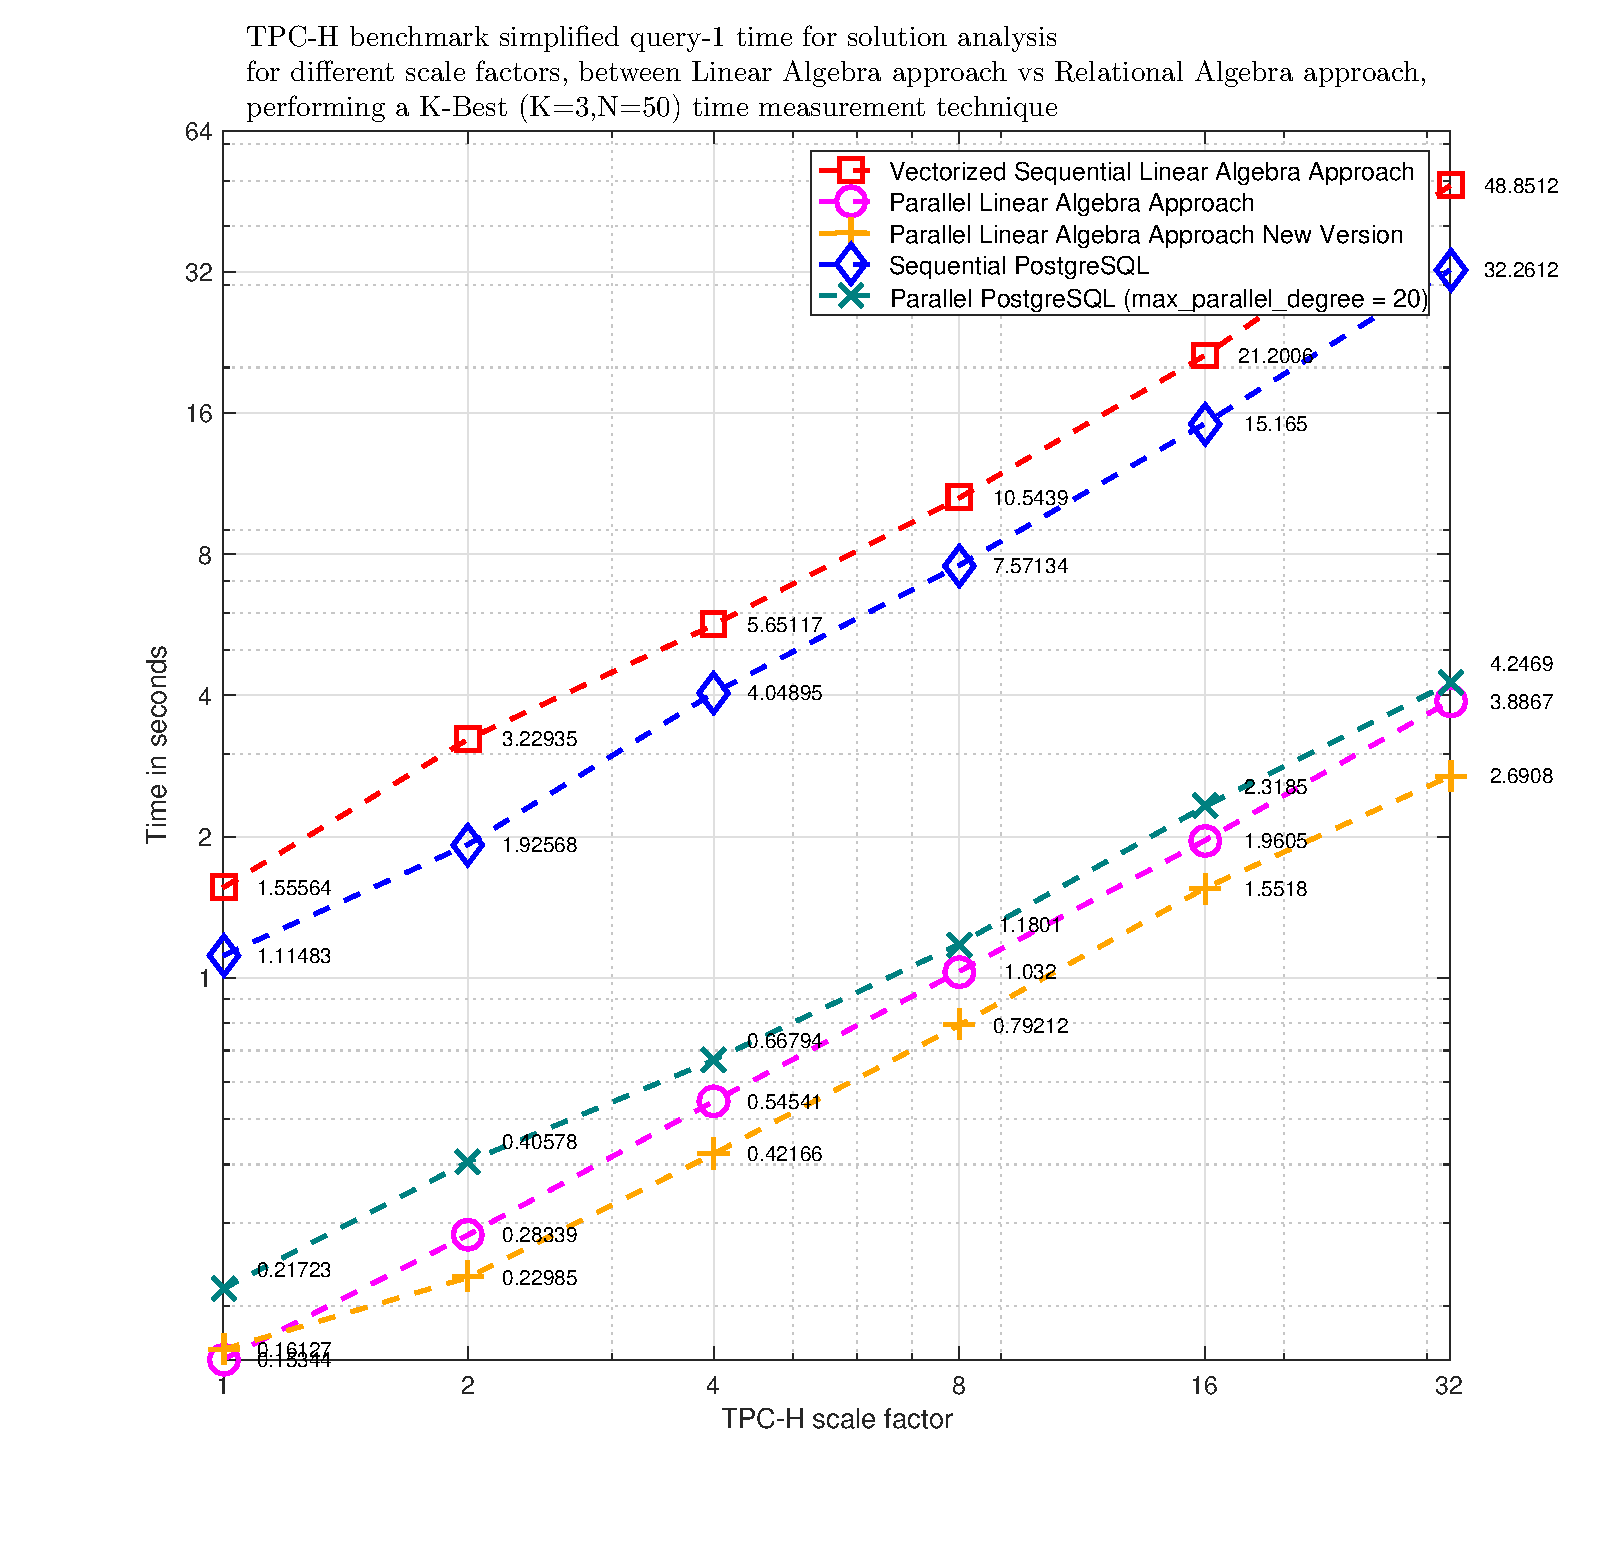
\includegraphics[width=0.95\columnwidth]{eps/TIME_LA_vs_RA_parallel_v2.eps}
\label{fig:time_la_vs_ra_parallel_v2}
\end{figure}


\begin{figure}[H]
\centering
\caption{TPC-H benchmark simplified query-1 speedup analysis for different scale factors, between sequential linear algebra vs parallel linear algebra and parallel linear algebra vs parallel relational algebra.}
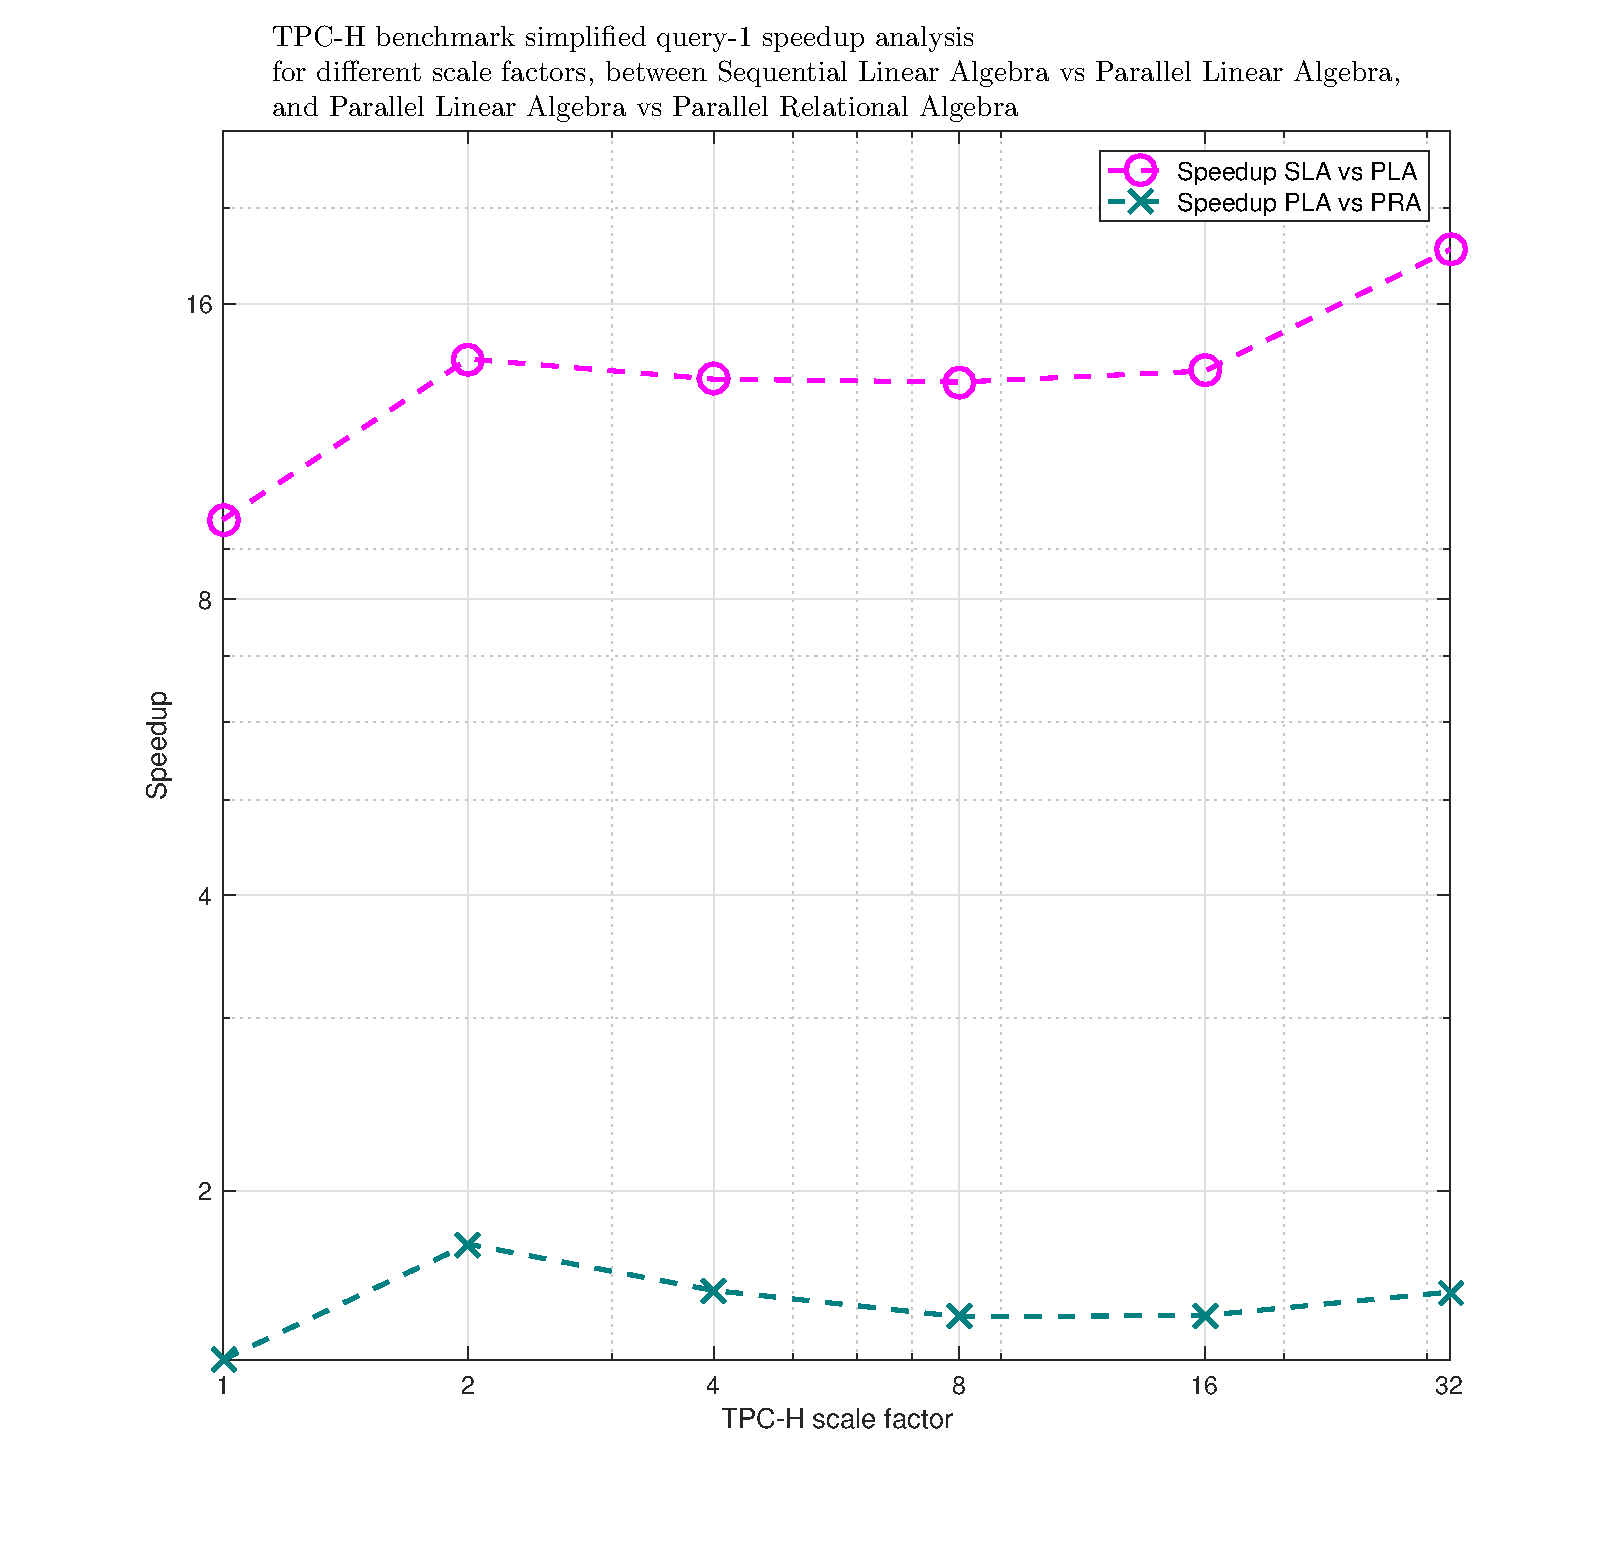
\includegraphics[width=0.95\columnwidth]{eps/speedup.eps}
\label{fig:speedup_la_vs_ra_parallel}
\end{figure}



